\documentclass[10pt]{beamer}

%STANDARD PREAMBLE
%https://tex.stackexchange.com/questions/68821/is-it-possible-to-create-a-latex-preamble-header
%\usepackage{/Users/mwojno01/Repos/latex_preamble/beamer_preamble}
\usepackage{/Users/miw267/Repos/csci246_spring2025/slides/preambles/beamer_preamble_for_CSCI246}


%%%
% SPECIFIC TO THIS DOCUMENT 
%%%
\let\warning\relax
\usepackage{fourier} % has warning  and danger symbols. However, it makes the bottoms tuff bold. 

\renewcommand{\ELBO}{\texttt{ELBO}}
\renewcommand{\Q}{\mathcal{Q}}


%%%%
% DOCUMENT 
%%%
\title{03/24/2026: Classic Diffusion Model}
\author{Reference: \textit{Deep unsupervised learning using nonequilibrium thermodynamics.}}
\date{CSCI 546: Diffusion Models}

\begin{document}
\maketitle

%\begin{frame}{Table of contents}
%  \setbeamertemplate{section in toc}[sections numbered]
%  \tableofcontents[hideallsubsections]
%\end{frame}

\begin{frame}{Table of contents}
  \setbeamertemplate{section in toc}[sections numbered]
  \setbeamertemplate{subsection in toc}[subsections numbered]
  \tableofcontents
\end{frame}


\section{Lab Overview}

\begin{frame}[standout]
Lab Overview
\end{frame}


\section{Course Logistics}



\begin{frame}
\begin{myredbox}[title=Announcements on syllabus]
Reminder: The syllabus is periodically updated! Always check the \blue{\underline{\href{https://github.com/mikewojnowicz/csci546_spring2026/blob/main/syllabus/syllabus.pdf}{syllabus in the repo.}}}
\vspace{.2cm}
\begin{itemize}
	\item The reading for Thursday has been shortened to Secs 20.1 and 20.2.
	\item The coding day for simple diffusion models has been moved up to next Tuesday.
\end{itemize}
\end{myredbox}
\end{frame}


\begin{frame}
\begin{mygreenbox}[title=Announcements on lightning chats (LC)]
\begin{itemize}
	\item LC assignments have been made. (See the \blue{\underline{\href{https://github.com/mikewojnowicz/csci546_spring2026/blob/main/syllabus/syllabus.pdf}{syllabus.}}})  
		\begin{itemize}
		\item If there's an \&, you're working together.  
		\item If there's a comma, there's some flexibility. I'd prefer you to work together (e.g. to save class time, to improve the quality of the product), but if you feel strongly about working separately, I'll likely make an exception. Please talk to your partner after class and let me know by Thursday. \pause 
		\item Note: Since the diffusion code day has moved up, some topic dates have shifted. \pause 
		\end{itemize} 
	\item Slide logistics 
		\begin{itemize}
		\item Please send a \alert{draft} of LC slides ahead of time, ideally the night before. I want to make sure I can open the slides. I may also provide some feedback.
		\item Please send final version by email sometime before class starts. \pause 
		\end{itemize}
	\item Content reminder 
		\begin{itemize}
		\item Could be anything... summary of the paper, your take on it, or a deep dive on some aspect of it (including background topic).
		\item Have fun with it! Goal is to provide an opportunity to learn and share your learning!
		\end{itemize}
\end{itemize}
\end{mygreenbox}
\end{frame}


\begin{frame}{Midterm Grades}

\begin{figure}
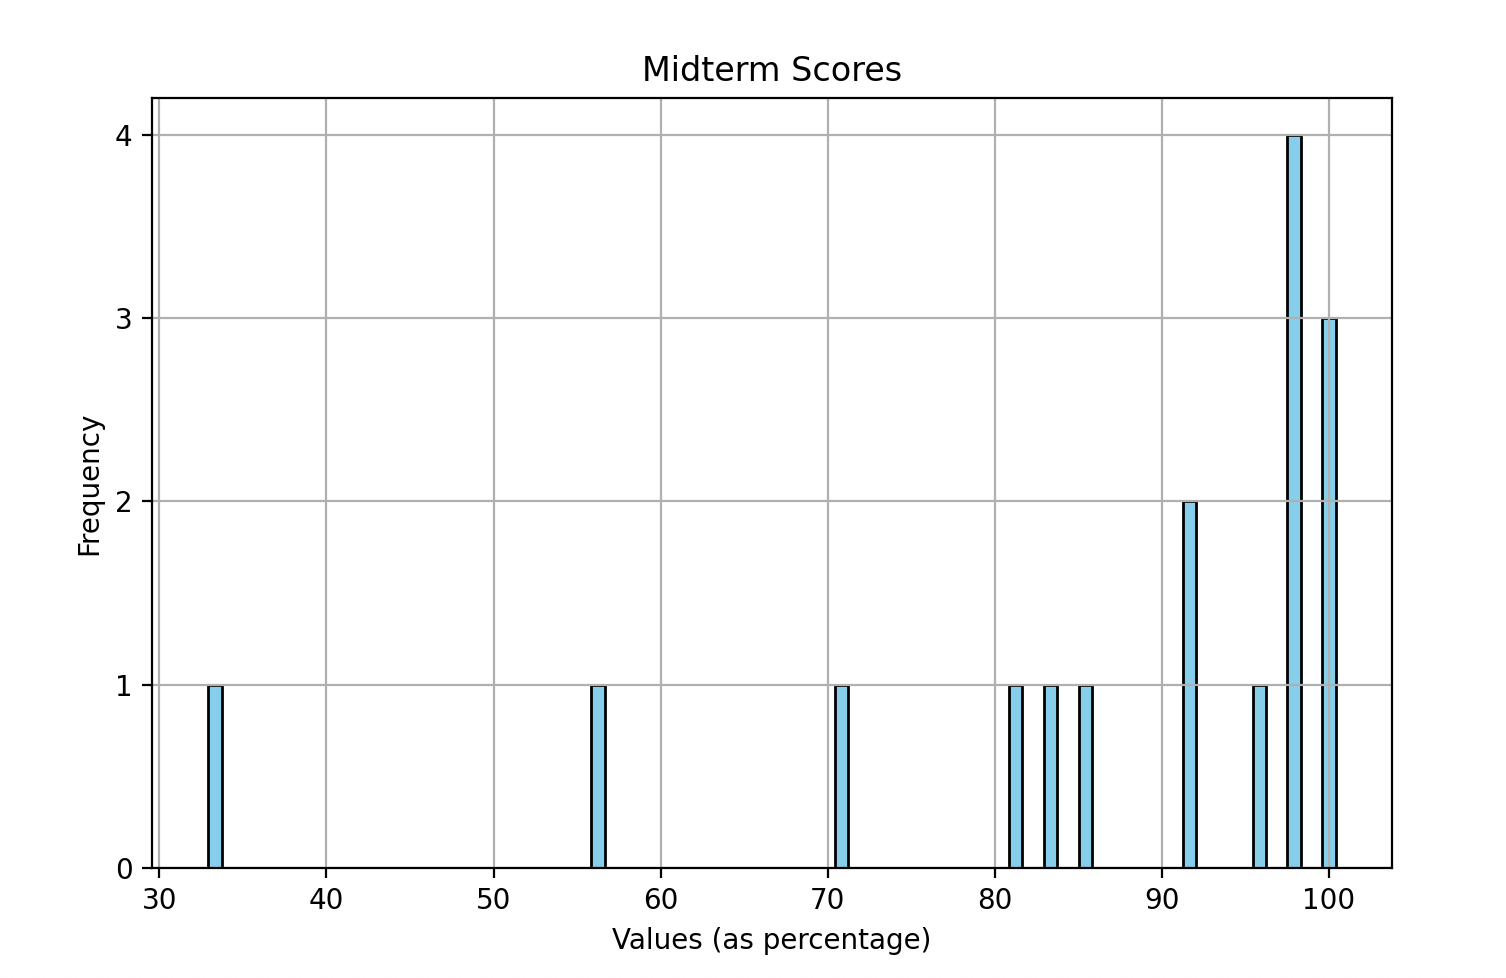
\includegraphics[width=\textwidth]{images/histogram}
\caption{Median Score: 93.75\%}
\end{figure}
\end{frame}




\begin{frame}
\begin{myredbox}[title=Announcements on grades]

\begin{itemize}
	\item Please let me know by email by Thursday if you'd like to retake the midterm, along with what time range you're thinking (so that I can sync up alternate versions). \pause
	\item Reminder:  Each version of the exam will re-draw questions from the original pool. \pause 
	\item If you are struggling with the material, please come to office hours or set up a 1-on-1 time. I want you to succeed!  Truly! \pause 
	\item Canvas has been updated with all grades so far: midterm, group exercise participation, and 2 reading surveys.
	\item I will return this material now.
\end{itemize}
\end{myredbox}
\end{frame}


\begin{frame}{Reading Survey}

\begin{enumerate}
	\item The paper proposes a method to flexibly learn complex probability distributions. Describe it.
\end{enumerate}
	
\end{frame}



\section{Lightning Chat}

\begin{frame}[standout]
Lightning Chat
\end{frame}

\section{Mini-Lecture}

\begin{frame}{Gaussian Diffusion}

\only<1>{
\begin{center}
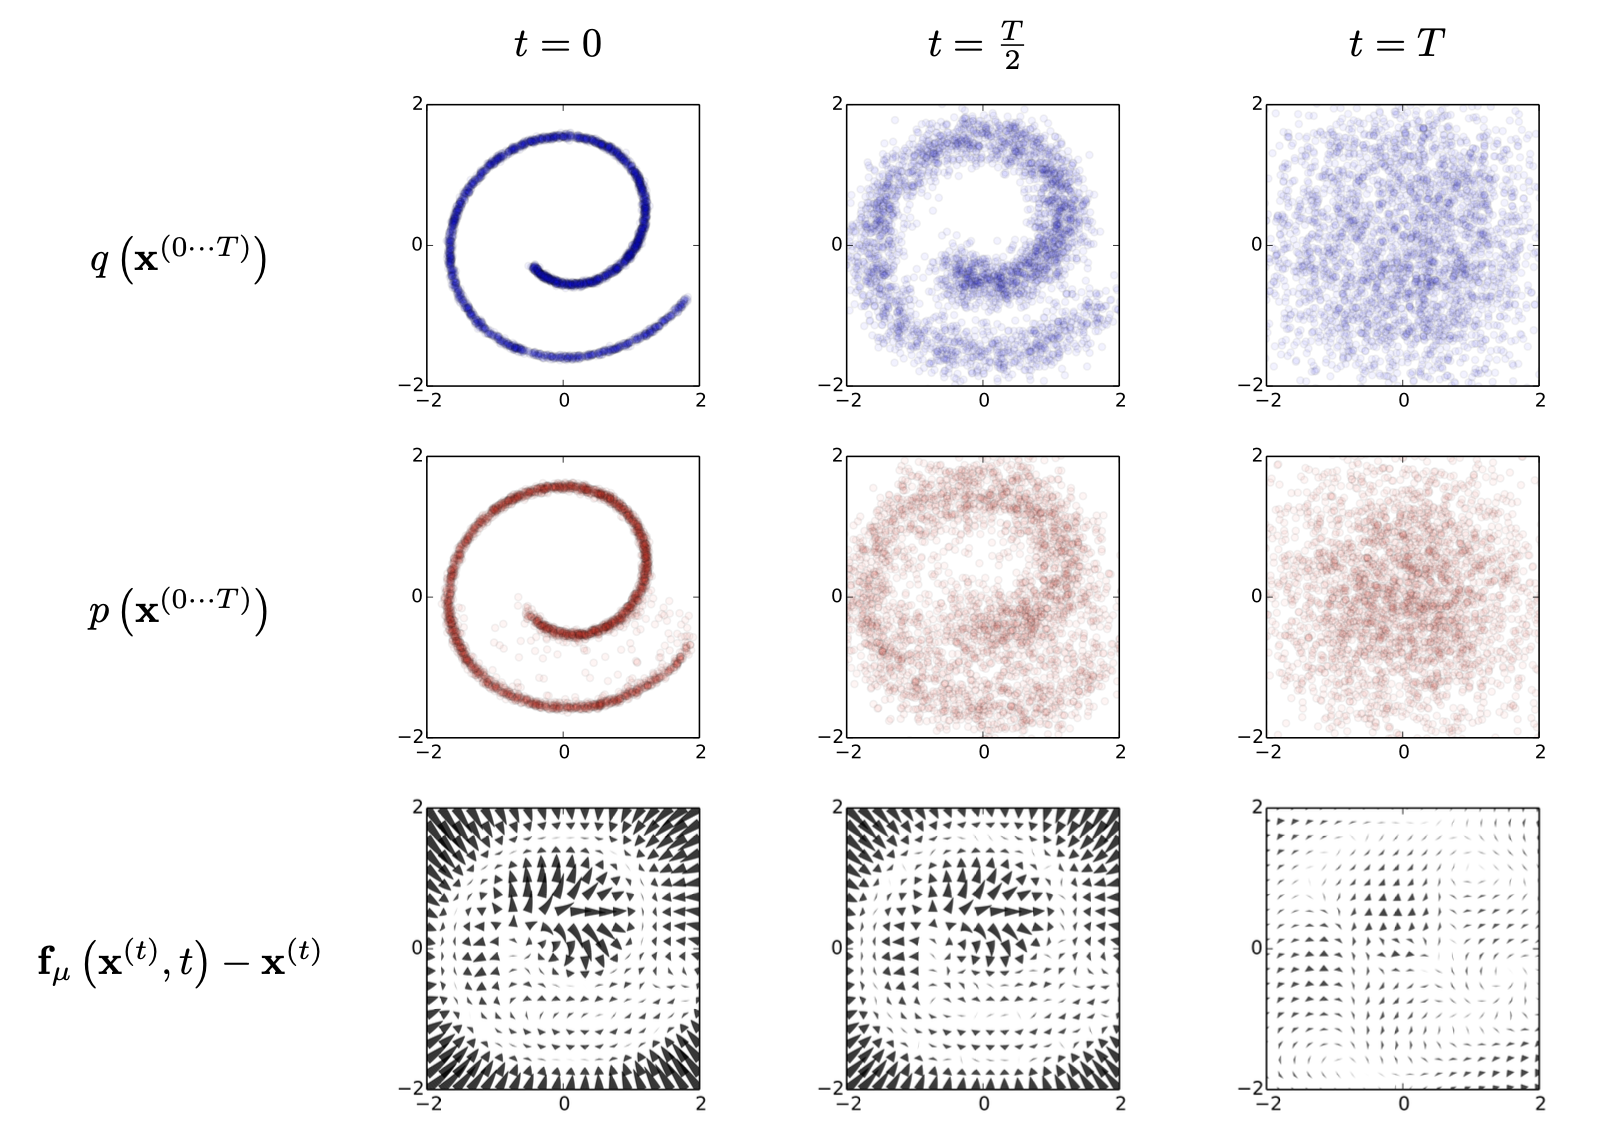
\includegraphics[width=\textwidth]{images/sohl_dickstein_2015_fig_1.png}	
\end{center}
}

\only<2-3>{

\begin{center}
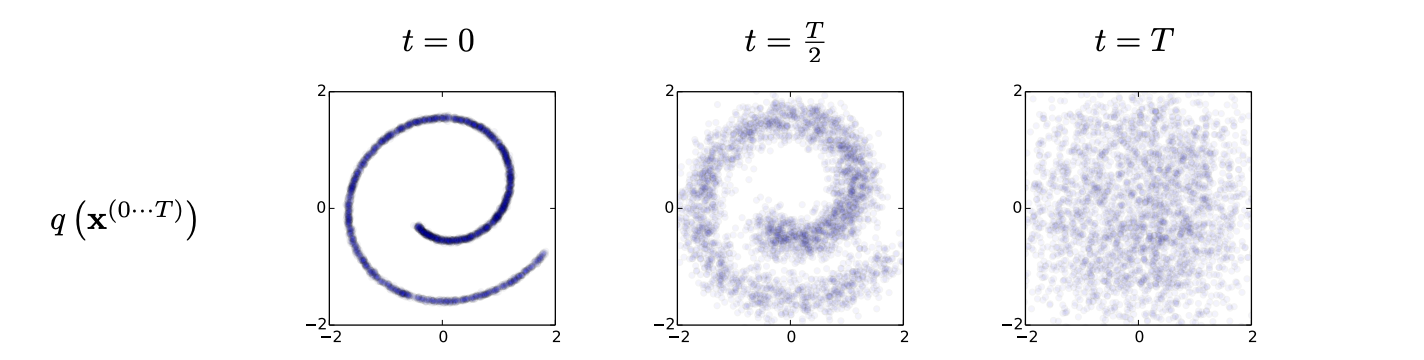
\includegraphics[width=\textwidth]{images/forward_process}	
\end{center}

\textbf{Forward trajectory.}

\begin{align*}
q\bigg(\+x^^{0 \hdots T}\bigg) &= 	q\bigg(\+x^^{0}\bigg) \prod_{t=1}^T q \bigg(\+x^^{t} \mid \+x^^{t-1} \bigg) 
\end{align*} 


\only<3>{
\vfill 
\colorbox{yellow!30}{\textbf{Poll.}} What do these factors represent?
}
}

\only<4>{

\begin{center}
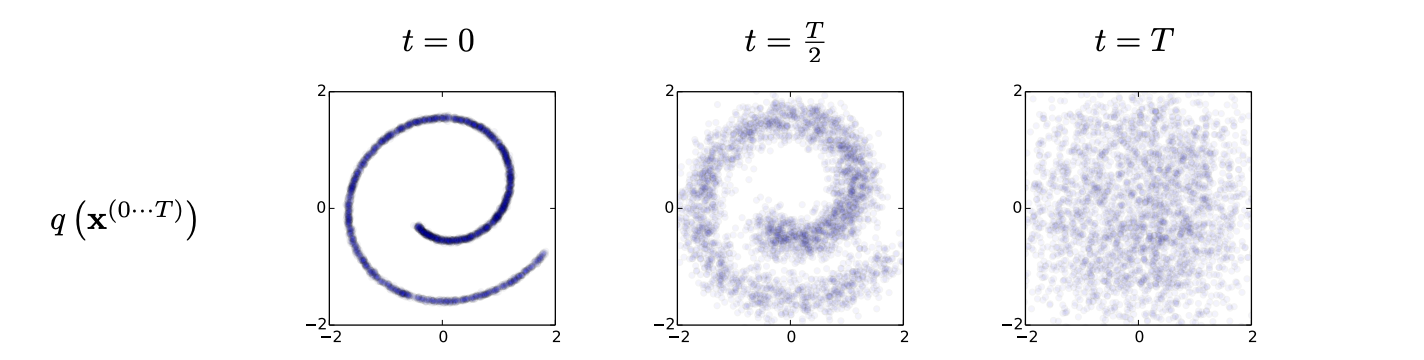
\includegraphics[width=\textwidth]{images/forward_process}	
\end{center}

\textbf{Forward trajectory.}

\begin{align*}
q\bigg(\+x^^{0 \hdots T}\bigg) &= 	\explaintermbrace{data dist.}{q\bigg(\+x^^{0}\bigg)} \; \prod_{t=1}^T \explaintermbrace{noise corruption}{q \bigg(\+x^^{t} \mid \+x^^{t-1} \bigg)} 
\end{align*}
}

\only<5->{

\begin{center}
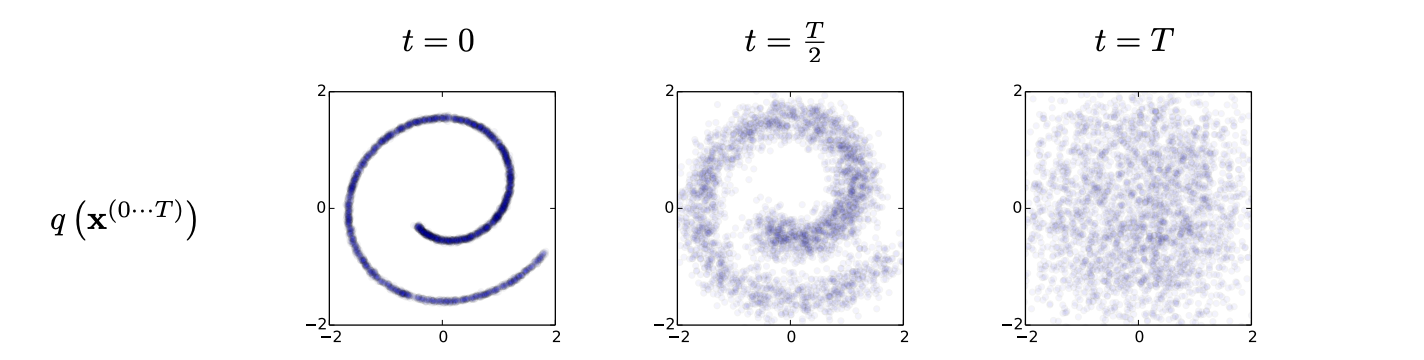
\includegraphics[width=.6\textwidth]{images/forward_process}	
\end{center}

\textbf{Forward trajectory.}

\begin{align*}
q\bigg(\+x^^{0 \hdots T}\bigg) &= 	\explaintermbrace{data dist.}{q\bigg(\+x^^{0}\bigg)} \; \prod_{t=1}^T \explaintermbrace{\alert{noise corruption}}{\alert{q \bigg(\+x^^{t} \mid \+x^^{t-1} \bigg)}}  \\
&\phantom{= q\bigg(\+x^^{0}\bigg) \; \prod_{t=1}^T}  \alert{\N \bigg(\+x^^{t} \,  ; \, \sqrt{1-\beta_t} \+x^^{t-1}, \+I \beta_t \bigg)} \\
&\phantom{= q\bigg(\+x^^{0}\bigg) \; \prod_{t=1}^T}  \qquad  \qquad \alert{\text{where } 0<\beta_t<1} 
\end{align*}

\only<6>{
\vfill 
\colorbox{yellow!30}{\textbf{Poll.}} As the number of diffusion steps $t$ increases, what happens to the mean? What happens to the structure?
}
}
\end{frame}



\begin{frame}{Gaussian Diffusion}


\only<1-2>{

\begin{center}
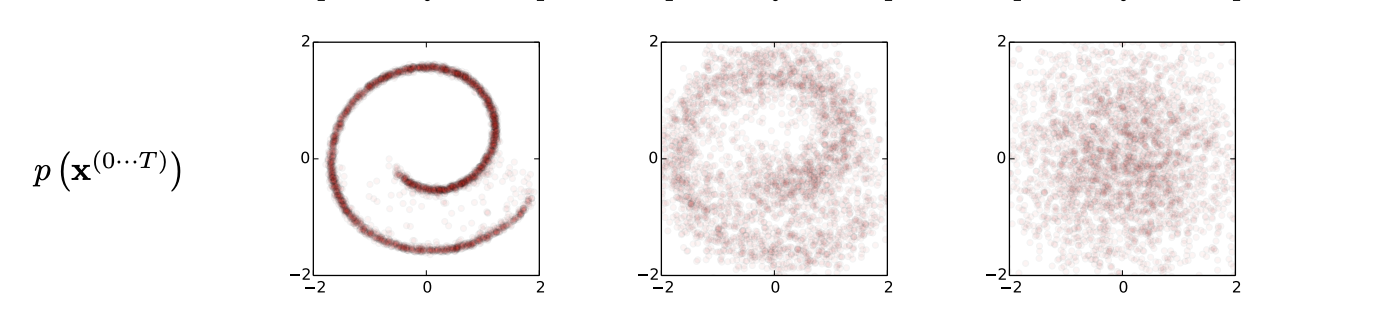
\includegraphics[width=\textwidth]{images/reverse_process}	
\end{center}

\textbf{Backward trajectory.}

\begin{align*}
p\bigg(\+x^^{0 \hdots T}\bigg) &= 	p\bigg(\+x^^{T}\bigg) \prod_{t=1}^T p\bigg(\+x^^{t-1} \mid \+x^^{t} \bigg) 
\end{align*} 


\only<2>{
\vfill 
\colorbox{yellow!30}{\textbf{Poll.}} What do these factors represent?
}
}

\only<3>{

\begin{center}
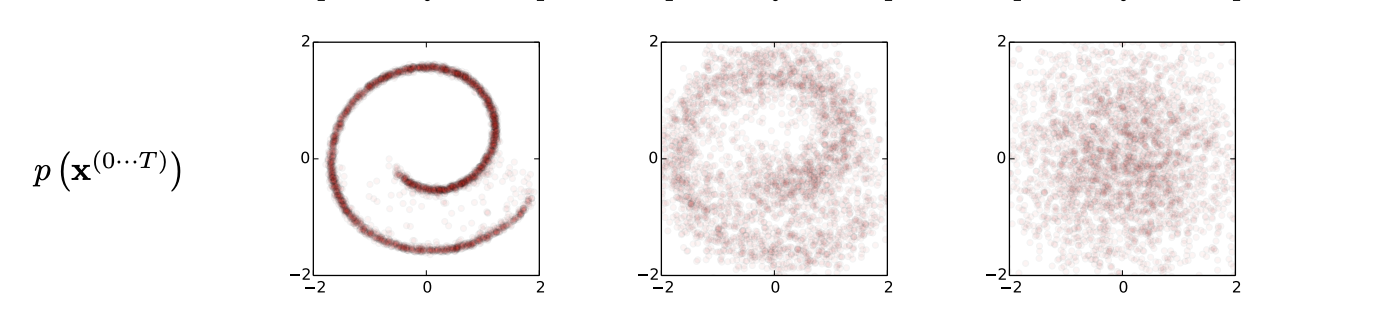
\includegraphics[width=\textwidth]{images/reverse_process}	
\end{center}

\textbf{Backward trajectory.}

\begin{align*}
p\bigg(\+x^^{0 \hdots T}\bigg) &= 	\explaintermbrace{Base distribution}{p\bigg(\+x^^{T}\bigg)} \, \prod_{t=1}^T \explaintermbrace{Denoising process}{p\bigg(\+x^^{t-1} \mid \+x^^{t}} \bigg) 
\end{align*} 
}

\only<4>{

\begin{center}
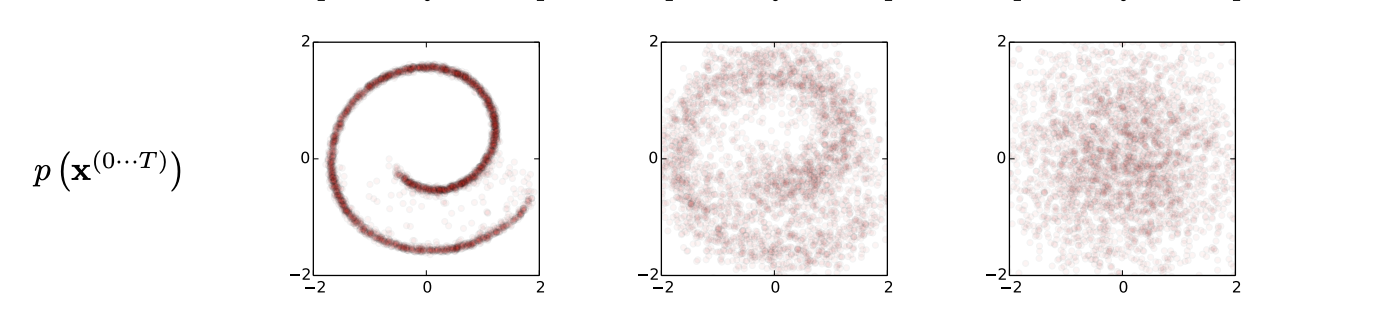
\includegraphics[width=.6\textwidth]{images/reverse_process}	
\end{center}

\textbf{Backward trajectory.}

\begin{align*}
p\bigg(\+x^^{0 \hdots T}\bigg) &= 	\explaintermbrace{\alert{Base distribution}}{\alert{p\bigg(\+x^^{T}\bigg)}} \, \prod_{t=1}^T \explaintermbrace{Denoising process}{p\bigg(\+x^^{t-1} \mid \+x^^{t}} \bigg)  \\
& \phantom{=} \alert{\N \bigg(\+x^^{t} \,  ; \, \+0, \+I\bigg)} \\
\end{align*}
}

\only<5>{

\begin{center}
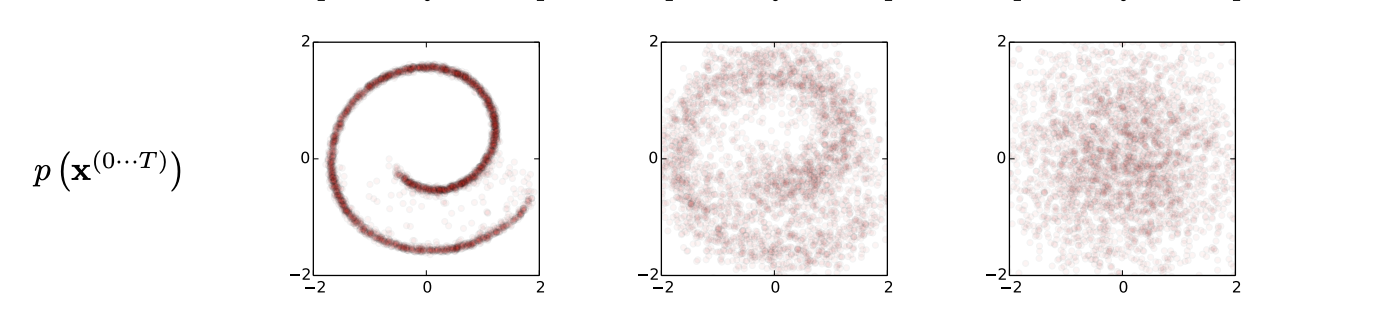
\includegraphics[width=\textwidth]{images/reverse_process}	
\end{center}

\textbf{Backward trajectory.}


\begin{align*}
p\bigg(\+x^^{0 \hdots T}\bigg) &= 	\explaintermbrace{Base distribution}{p\bigg(\+x^^{T}\bigg)} \, \prod_{t=1}^T \explaintermbrace{\alert{Denoising process}}{\alert{p\bigg(\+x^^{t-1} \mid \+x^^{t}} \bigg)} \\
& \phantom{= 	\explaintermbrace{Base distribution}{p\bigg(\+x^^{T}\bigg)} \, \prod_{t=1}^T} \alert{\N \bigg(\+x^^{t-1} \,  ; \, \+f_\mu \big(\+x^^{t}, t \big),  \+f_\Sigma \big(\+x^^{t}, t \big) \bigg)} \\[-2em]
& \phantom{= 	\explaintermbrace{Base distribution}{p\bigg(\+x^^{T}\bigg)} \, \prod_{t=1}^T} \alert{\qquad \qquad \text{where } \+f_\mu, \+f_\Sigma \; \text{ are MLPs} } \\ 
\end{align*} 
}

\end{frame}






\begin{frame}{Binomial Diffusion}

\only<1-4>{
\begin{center}
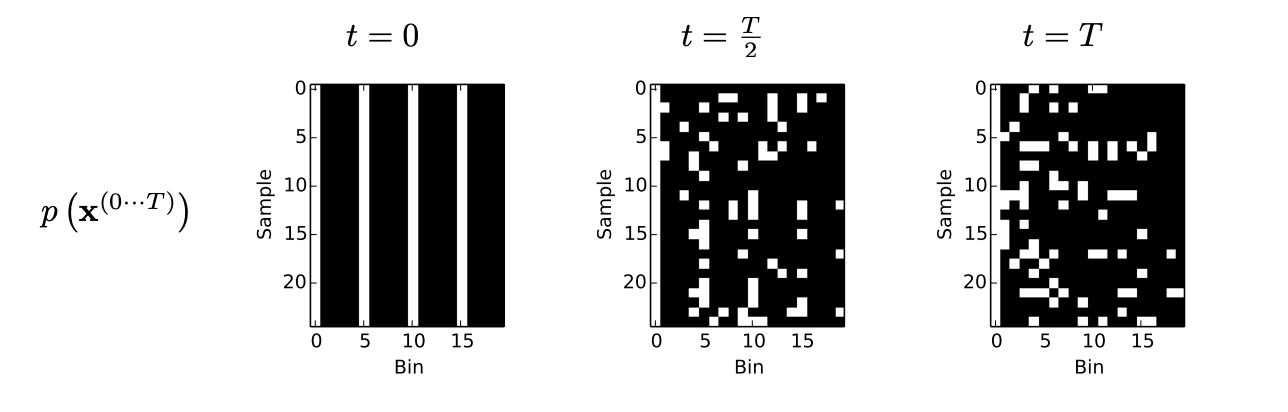
\includegraphics[width=\textwidth]{images/binomial_diffusion}	
\end{center}
}

\only<2-3>{

\textbf{Forward trajectory.}

\begin{align*}
q\bigg(\+x^^{0 \hdots T}\bigg) &= 	q\bigg(\+x^^{0}\bigg) \prod_{t=1}^T q \bigg(\+x^^{t} \mid \+x^^{t-1} \bigg) 
\end{align*} 
}

\only<3>{
\vfill 
\colorbox{yellow!30}{\textbf{Poll.}} What do these factors represent?
}


\only<4>{


\textbf{Forward trajectory.}

\begin{align*}
q\bigg(\+x^^{0 \hdots T}\bigg) &= 	\explaintermbrace{data dist.}{q\bigg(\+x^^{0}\bigg)} \; \prod_{t=1}^T \explaintermbrace{noise corruption}{q \bigg(\+x^^{t} \mid \+x^^{t-1} \bigg)} 
\end{align*}
}

\only<5->{

\begin{center}
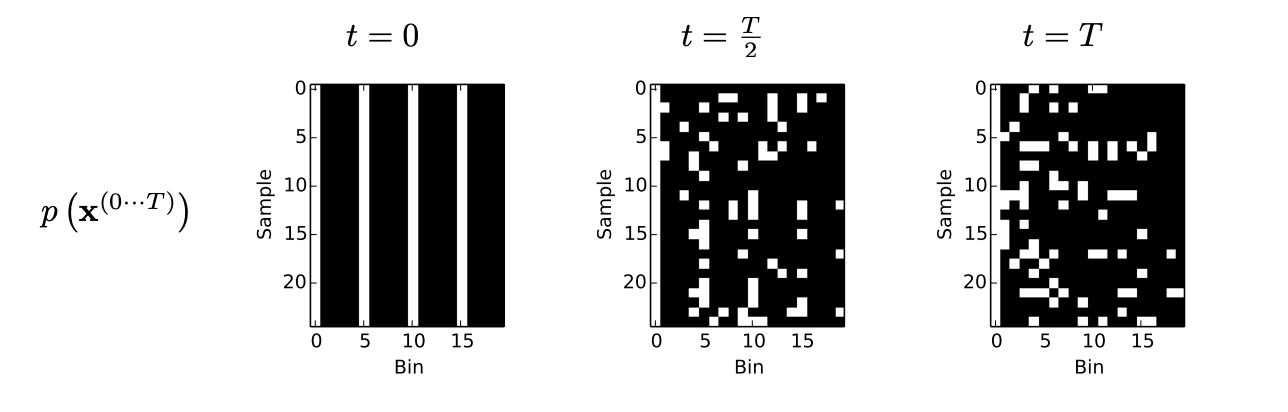
\includegraphics[width=.7\textwidth]{images/binomial_diffusion}	
\end{center}


\textbf{Forward trajectory.}

\begin{align*}
q\bigg(\+x^^{0 \hdots T}\bigg) &= 	\explaintermbrace{data dist.}{q\bigg(\+x^^{0}\bigg)} \; \prod_{t=1}^T \explaintermbrace{\alert{noise corruption}}{\alert{q \bigg(\+x^^{t} \mid \+x^^{t-1} \bigg)}}  \\
&\phantom{= q\bigg(\+x^^{0}\bigg) \; \prod_{t=1}^T}  \alert{\mathcal{B} \bigg(\+x^^{t} \,  ; \, (1-\beta_t) \+x^^{t-1} \, + \, \beta_t 0.5 \bigg)} \\[-1em]
&\phantom{= q\bigg(\+x^^{0}\bigg) \; \prod_{t=1}^T}  \qquad  \qquad \alert{\text{where } 0<\beta_t<1} 
\end{align*}

\only<6>{
\vfill 
\colorbox{yellow!30}{\textbf{Poll.}} As the number of diffusion steps $t$ increases, what happens to the mean? What happens to the structure?
}
}
\end{frame}

\begin{frame}{Equilibrium Distribution}
\small 
\only<1->{
These diffusions are \alert{Markov chains} which eventually reach an equilibrium distribution.
}  
\only<2->{
\vfill
E.g., for Gaussian diffusion, the \textbf{transition kernel} is given by
\[ q \bigg(\+y \mid \+y' \bigg) :=  \N \bigg(\+y \,  ; \, \sqrt{1-\beta_t} \+y', \+I \beta_t \bigg) \] 
}
\only<3->{
\vfill
The \alert{equilibrium distribution} is 
\[ \pi(\+y) =  \N \bigg(\+0, \+I \bigg) \]
}
\only<4->{ 
That is, we have
\[ \pi(\+y) = \int d\+y'  \pi(\+y') q(\+y \mid \+y') \]
}
\only<5-6>{
\colorbox{yellow!30}{\textbf{Poll.}} How is this related to equilibrium distributions on finite state spaces?
}
\only<6-7>{
\colorbox{blue!30}{\textbf{Recall.}} For Markov chains on finite state spaces with t.p.m. $\+P$, an equilibrium distribution was defined by
\begin{align*}
\+\pi &= \+\pi \+P \\
\implies \pi_j &= \sum_i \pi_i \+P_{ij}	
\end{align*}
}
\only<7>{
So either way, we're ``integrating'' over possible starting values.
}

\end{frame}



\section{Group Work}


\begin{frame}{Group Exercises}

\begin{enumerate}
	\item How do we know that if we define the forward process via the transition kernel $q(\+x_t \cond \+x_{t-1}) = \N(\+x_t; \sqrt{1-\beta_t} \+x_{t-1}, \beta_t \+I)$ that there is an equilibrium distribution, and moreover that the equilibrium distribution is $\pi = \N(\+0, \+I)$?
\end{enumerate} 

\vfill 
\pause 
\textit{Hint:} (Assuming that the kernel is aperiodic and $\pi$-irreducible), it suffices to verify detailed balance:

That is, we must show 
\[ \pi(y) q(x \cond y) \stackrel{?}{=} \pi(x) q(y \cond x) \] 

	
\end{frame}

\begin{frame}{Good, Bad, Ugly, Beautiful}

\textbf{Guidelines}
Fill this out
\begin{enumerate}
	\item \textit{Good, Bad}: Technical content
	\item \textit{Ugly, Beautiful}: Presentational styles
\end{enumerate}

\vfill 


\textbf{Format}
\begin{enumerate}
	\item Small group discussion  \alert{at whiteboards}.  (Fill out your responses there.)
	\item Class discussion 
\end{enumerate}
	
\end{frame}

\begin{frame}{Random groups}
\begin{columns}
\begin{column}{0.33\textwidth}
Aubrey Williams: 8 \\ 
Austin Barton : 5 \\ 
Blake Sigmundstad: 6 \\ 
Diego Moylan: 7 \\ 
Dillon Shaffer: 7 \\ 
Ismoiljon Muzaffarov: 2 \\ 
Jacob Tanner: 1 \\\end{column}
\begin{column}{0.33\textwidth}
Josh Stoneback: 8 \\ 
Joshua Bowen: 6 \\ 
Joshua Culwell: 4 \\ 
Laura Banaszewski: 4 \\ 
Lina Hommel: 5 \\\end{column}
\begin{column}{0.33\textwidth}
Logan Racz: 1 \\ 
Matt Hall: 2 \\ 
Mike Kadoshnikov: 2 \\ 
Owen Cool: 3 \\ 
Racquel Bowen: 1 \\ 
Samuel Mocabee: 3 \\ 
Tatiana Kirillova: 3 \\\end{column}
\end{columns}	
\end{frame}





\end{document}

